%% May 2016, 
%presentation inspired by the presentation made in CAA, the presentation made at the Winter Simulation Conference, and some ideas tooks from #RIN4 at the UPF

\documentclass[12pt, notes=show]{beamer}
\usetheme[width=0cm]{Goettingen}
\usecolortheme{rose}
\useoutertheme{default}
\setbeamerfont{caption}{size=\scriptsize}
\setbeamertemplate{navigation symbols}{}

\addtobeamertemplate{navigation symbols}{}{%
	\usebeamerfont{footline}%
	\usebeamercolor[fg]{footline}%
	\hspace{1em}%
	$\dfrac{\insertframenumber}{\inserttotalframenumber}$
}

\usepackage{hyperref}
\usepackage{fontspec} 
%\setsansfont{Futura LT}


\usepackage{arydshln}
\usepackage{amsmath}
\usepackage{multicol}

\usepackage{mathptmx}
\usepackage{latexsym}
\usepackage{mathtools}
\usepackage{multirow}
\usepackage{caption}


\newcommand{\compresslist}{
    \setlength{emsep}{1pt}
    \setlength{\parskip}{0pt}
    \setlength{\parsep}{0pt}
}
\begin{document}


\begin{frame}{A General Agent Based Framework }

     Two main components:
     \vfill
    \begin{enumerate}
	\item Trade side: Bartering Economy,
	\item Cultural side: innovation and social learning.
    \end{enumerate}
    \begin{center}
	\includegraphics[width=.8\textwidth]{../201605_BSC2/images/interaction}	
    \end{center}
\end{frame}

\begin{frame}{The Model}
	\begin{block}{1. The Economy \& the Barter Mechanism}
		\begin{itemize}
			\item $N$ goods
			\item $M$ Agent 
				$\left\{
					\begin{tabular}{@{}l@{}}
						a quantity of each Goods \\
						$N$ values attributed to each goods\\
					\end{tabular}
					\right.$
				\item Agents \emph{produce} one good and \emph{exchange} it to obtain the other goods.
				\item After the exchange, the agents \emph{consume} all goods 
			\end{itemize}
			Agent perform this 10 times and a scores is given to each of them.
		\end{block}
	\end{frame}

	\begin{frame}{The Model}
		\begin{block}{2. Cultural Mechanisms}
			\begin{itemize}
					\vfill
				\item Less successful agents \emph{copy} the most successful (Biased-Copy).
					\vfill
				\item Given a probability $\mu$ the value attributed to some goods is modified (Innovation/Mutation)
			\end{itemize}
		\end{block}
	\end{frame}
	\begin{frame}{General Equilibrium}
	    \begin{quotation}
		\footnotesize
		Given initial endowment $w_i$, consumers \& producers use prices $p_i$ that allow to produce, exchange and consume goods from markets $i$ in such quantities $x_i$ that nothing is missing nor left in the markets (\emph{``market-clearing prices''}). 
	    \end{quotation}
	    \begin{itemize}
		\item  Consumers are buying the exact quantities of goods they want (utility maximization). 
		\item  Producer are maximizing their profit.
	    \end{itemize}

	    Walras: equilibrium reached by ``tâtonnement'' process, done by an auctioneer with perfect knowledge of everything.

	\end{frame}



\begin{frame}{Equilibrium}
    \begin{figure}[!h]
	\centering
	\begin{tabular}{ c c}
	    Scores & Prices \\
	    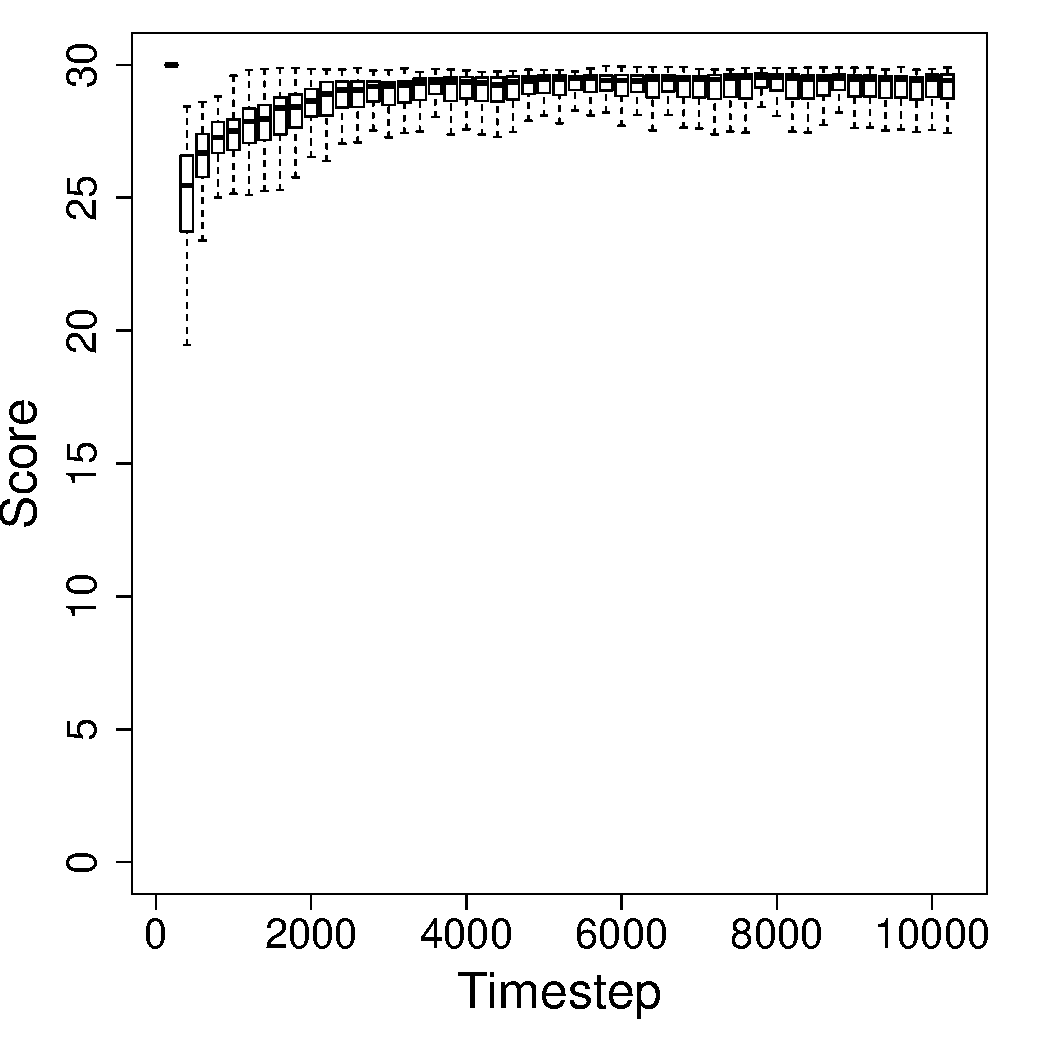
\includegraphics[width=5cm]{../20160329_CAA/images/ScoreEvolutionForTrade-G3N500.pdf}
	    & \
		\includegraphics[width=5cm]{../20160329_CAA/images/ClearingPriceDistanceEvolutionForTrade-G3N500.pdf}\\

	\end{tabular}
	\label{fig:scoreEvol}
    \end{figure}
\end{frame}

\begin{frame}{Explore the model}

    Conditions that lead to equilibrium?

     \vfill
    \begin{enumerate}
	\item Trade side: Type of economy, trade network\dots 
	\item Cultural side: Innovation rate, social network (Complenet16), social learning strategies\dots
    \end{enumerate}
    \begin{center}
	\includegraphics[width=.8\textwidth]{../201605_BSC2/images/interaction}	
    \end{center}
\end{frame}



	\begin{frame}{Approximate Bayesian Computation}

	    Compute likelihood of models to ``explain'' empirical evidences (Rubio-Campillo 2016):
	    \begin{figure}[H]
		\begin{center}
		    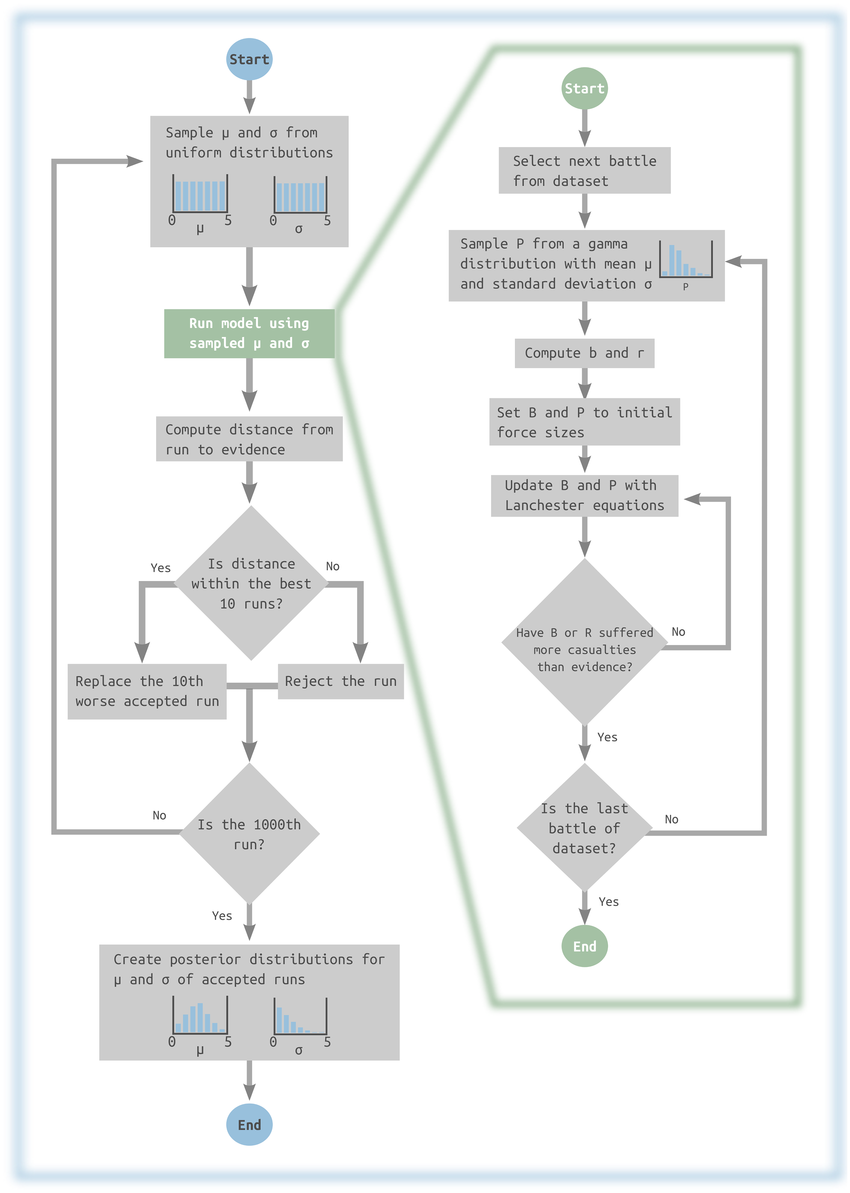
\includegraphics[height=.7\textheight]{Fig-4-Flowchart-for-the-ABC-frameworkExample-for-a-experiment-using-1000-runs-and.png}
		\end{center}
	    \end{figure}
	    

	\end{frame}

	\begin{frame}{Slight variation: FIO}

	    {	     Fitting to idealized outcomes:
		\small
		 \begin{enumerate}
		     \item  sample of $\mu$ with $\mu\sim U(0,1)$
		     \item  run simulations with innovation rate = $\mu$ 
		     \item  compute distance $\epsilon$ to idealize outcome~(GE):  
			 \begin{align*}
			     \epsilon = \frac{ \sum_{i=1}^{n} s_i-s_{ge} }{n}   
			 \end{align*}
			 {\tiny ($n$: total number of agents, $s_i$ score of agent i, $s_{ge}$: ideal score)}
			 \vfill
		     \item  select $200$ simulations with $\epsilon<.25$, 
		     \item  draw \emph{posterior} distribution of $\mu$ for those simulations.
		 \end{enumerate}
	     }
		 \begin{center}
		     \textbf{
		     Our idealized outcome:\\ General Equilibrium $\rightarrow$ $s_{ge}=0$
		 }
		 \end{center}

	\end{frame}


	\begin{frame}{Innovation Process}
	    Focus on one part of the model
		\begin{block}{2. Cultural Mechanisms}
			\begin{itemize}
					\vfill
				\item Less successful agents \emph{copy} the most successful (Biased-Copy).
					\vfill
				\textbf{\item Given a probability $\mu$ the value attributed to some goods is modified (Innovation/Mutation)}
			\end{itemize}
		\end{block}
	\end{frame}
    
	\begin{frame}{Innovation Process}

	    \begin{figure}[H]
		\begin{center}
		    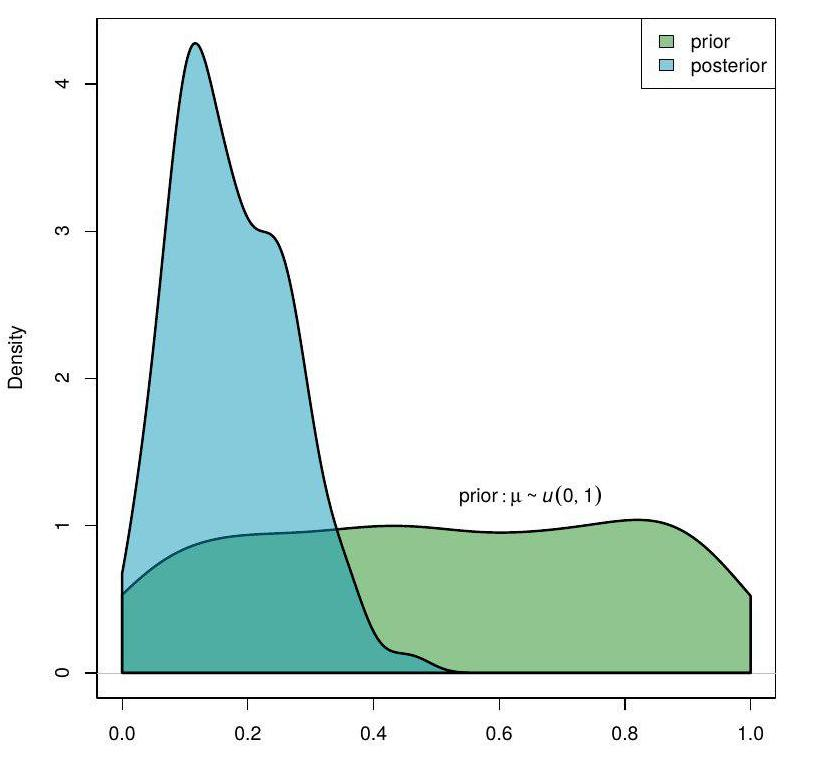
\includegraphics[height=.8\textheight]{ABC.jpg}
		\end{center}
	    \end{figure}
	    

	\end{frame}
\end{document}



